\documentclass[a4paper,twoside]{article}
\usepackage{blindtext}  
\usepackage{geometry}

% Chinese support
\usepackage[UTF8, scheme = plain]{ctex}

% Page margin layout
\geometry{left=2.3cm,right=2cm,top=2.5cm,bottom=2.0cm}


\usepackage{listings}
\usepackage{xcolor}
\usepackage{geometry}
\usepackage{amsmath}
\usepackage{float}
\usepackage{hyperref}

\usepackage{graphics}
\usepackage{graphicx}
\usepackage{subcaption}
\usepackage{epsfig}
\usepackage{float}

\usepackage{algorithm}
\usepackage[noend]{algpseudocode}

\usepackage{booktabs}
\usepackage{threeparttable}
\usepackage{longtable}
\usepackage{tabularx}
\usepackage{tikz}
\usepackage{multicol}
\usepackage{pgfplots}
\pgfplotsset{compat=1.9}
\pgfplotsset{
    myplotstyle/.style={
    legend style={draw=none, font=\small},
    legend cell align=left,
    legend pos=north east,
    ylabel style={align=center, font=\bfseries\boldmath},
    xlabel style={align=center, font=\bfseries\boldmath},
    x tick label style={font=\bfseries\boldmath},
    y tick label style={font=\bfseries\boldmath},
    scaled ticks=false,
    every axis plot/.append style={thick},
    },
}

% cite package, to clean up citations in the main text. Do not remove.
\usepackage{cite}

\usepackage{color,xcolor}

%% The amssymb package provides various useful mathematical symbols
% \usepackage{amssymb}
%% The amsthm package provides extended theorem environments
% \usepackage{amsthm}
% \usepackage{amsfonts}
\usepackage{enumerate}
\usepackage{enumitem}
\usepackage{listings}
\usepackage{minted}


\usepackage{indentfirst}
\setlength{\parindent}{2em} % Make two letter space in the first paragraph
\usepackage{setspace}
\linespread{1.5} % Line spacing setting
\usepackage{siunitx}
\setlength{\parskip}{0.5em} % Paragraph spacing setting

% \usepackage[contents =22920202204622, scale = 10, color = black, angle = 50, opacity = .10]{background}

\renewcommand{\figurename}{图}
\renewcommand{\listingscaption}{代码}
\renewcommand{\tablename}{表格}
\renewcommand{\contentsname}{目录}
\floatname{algorithm}{算法}

\graphicspath{ {images/} }

%%%%%%%%%%%%%
\newcommand{\StudentNumber}{22920202204622}  % Fill your student number here
\newcommand{\StudentName}{熊恪峥}  % Replace your name here
\newcommand{\PaperTitle}{实验(六)}  % Change your paper title here
\newcommand{\PaperType}{实验报告} % Replace the type of your report here
\newcommand{\Date}{2023年6月13日}
\newcommand{\College}{信息学院}
\newcommand{\CourseName}{数据库}
%%%%%%%%%%%%%

%% Page header and footer setting
\usepackage{fancyhdr}
\usepackage{lastpage}
\pagestyle{fancy}
\fancyhf{}
% This requires the document to be twoside
\fancyhead[LO]{\texttt{\StudentName }}
\fancyhead[LE]{\texttt{\StudentNumber}}
\fancyhead[C]{\texttt{\PaperTitle }}
\fancyhead[R]{\texttt{第{\thepage}页,共\pageref*{LastPage}页}}


\title{\PaperTitle}
\author{\StudentName}
\date{\Date}

\algnewcommand\algorithmicinput{\textbf{Input:}}
\algnewcommand\algorithmicoutput{\textbf{Output:}}
\algnewcommand\Input{\item[\algorithmicinput]}%
\algnewcommand\Output{\item[\algorithmicoutput]}%

\usetikzlibrary{positioning, shapes.geometric}

\begin{document}
	
%%%%%%%%%%%%%%%%%%%%%%%%%%%%%%%%%%%%%%%%%%%%
\makeatletter % change default title style
\renewcommand*\maketitle{%
	\begin{center} 
		\bfseries  % title 
		{\LARGE \@title \par}  % LARGE typesetting
		\vskip 1em  %  margin 1em
		{\global\let\author\@empty}  % no author information
		{\global\let\date\@empty}  % no date
		\thispagestyle{empty}   %  empty page style
	\end{center}%
	\setcounter{footnote}{0}%
}
\makeatother
%%%%%%%%%%%%%%%%%%%%%%%%%%%%%%%%%%%%%%%%%%%%
	
	
\thispagestyle{empty}

\vspace*{1cm}

\begin{figure}[htb]
	\centering
	
\includegraphics[width=4.0cm]{logo.png}
\end{figure}

\vspace*{1cm}

\begin{center}
	\Huge{\textbf{\PaperType}}
	
	\Large{\PaperTitle}
\end{center}

\vspace*{1cm}

\begin{table}[h]
	\centering	
	\begin{Large}
		\renewcommand{\arraystretch}{1.5}
		\begin{tabular}{p{3cm} p{5cm}<{\centering}}
			姓\qquad 名 & \StudentName  \\
			\hline
			学\qquad号 & \StudentNumber \\
			\hline
			日\qquad期 & \Date  \\
			\hline
			学\qquad院 & \College  \\
			\hline
			课程名称 & \CourseName  \\
			\hline
		\end{tabular}
	\end{Large}
\end{table}

\newpage

\title{
	\Large{\textcolor{black}{\PaperTitle}}
}
	
	
\maketitle
	
\tableofcontents
 
\newpage
\setcounter{page}{1}

\begin{spacing}{1.2}

\section{实验目的}
通过本次实验,要求掌握变量定义,流程控制,存储过程,存储函数,游标等内容。

\section{实验内容}
\begin{enumerate}
  \item 变量的声明和使用,掌握@@ERROR、@@ROWCOUNT、@@IDENTITY等全局变量的使用。2. 使用BEGIN…END、IF…ELSE…、 WHILE…CONTINUE…BREAK…、CASE等流程控制语句。
  \item 使用存储过程。
  \item 使用系统函数和用户自定义函数。
  \item 使用游标处理数据。
\end{enumerate}

\section{实验步骤}

\begin{enumerate}
  \item 用T-SQL语言完成$1+2+3+\ldots+100$,并使用@@ERROE判断是否执行成功,如果成功则输出值,否则打印执行失败。
\inputminted[firstline=3,lastline=19]{sql}{../code/1.sql}
\begin{figure}[h]
  \centering
  \caption{运行结果}
  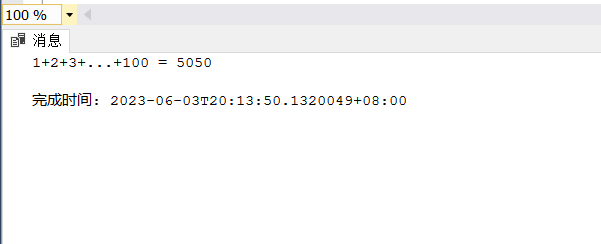
\includegraphics[width=0.4\textwidth]{images/1.png}
\end{figure}
  \item 更新STUDENTS表中sid为80000759500的学生的email为ddff@sina.com,并通过@@ROWCOUNT判断是否有数据被更新,如果没有则打印警告。
\inputminted[firstline=23,lastline=49]{sql}{../code/1.sql}
\begin{figure}[h]
  \centering
  \caption{运行结果}
  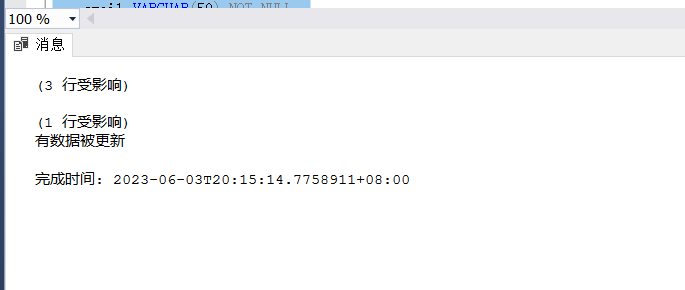
\includegraphics[width=0.4\textwidth]{images/2.png}
\end{figure}
  \item 使用IF…ELSE…语句,查询STUDENTS表中学号为800007595的学生,如果学生存在,则输出学生的各科成绩,否则打印查无此人。
\inputminted[firstline=56,lastline=92]{sql}{../code/1.sql}
\begin{figure}[h]
  \centering
  \caption{运行结果}
  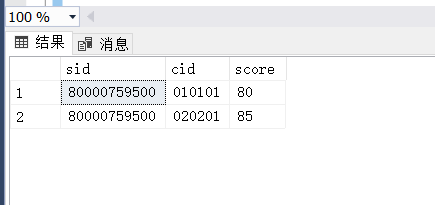
\includegraphics[width=0.4\textwidth]{images/3.png}
\end{figure}
  \item 使用WHILE语句计算$1+2+3+\ldots+100$
\inputminted[firstline=95,lastline=104]{sql}{../code/1.sql}
\begin{figure}[h]
  \centering
  \caption{运行结果}
  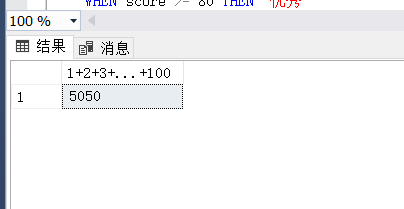
\includegraphics[width=0.4\textwidth]{images/4.png}
\end{figure}
  \item 使用CASE语句,查询学号为800007595所选择的课程号为10042的成绩,如果为80分或以上,打印优秀,如果在60—80分之间则打印及格,否则打印不及格。
\inputminted[firstline=108,lastline=114]{sql}{../code/1.sql}
\begin{figure}[h]
  \centering
  \caption{运行结果}
  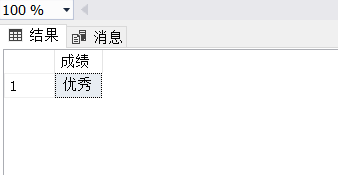
\includegraphics[width=0.4\textwidth]{images/5.png}
\end{figure}
  \item 使用T-SQL命令CREATE PROC语句可创建存储过程,创建一个带输入和输出参数的存储过程,查询学生选修课程成绩,将分数低于60分的成绩改为60分,高于80分的成绩改为80分。输入参数为学生的学号,输出参数为提示信息,如果不学生不存在则参数值为查无此人,更改失败则为更改失败,更改成功则为更改成功。
\begin{figure}[h]
  \centering
  \caption{运行结果}
  \begin{subfigure}{0.4\textwidth}
    \caption{输出消息}
    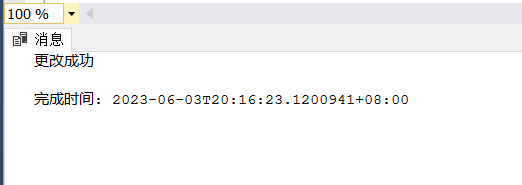
\includegraphics[width=0.9\textwidth]{images/6.png}
  \end{subfigure}
  \begin{subfigure}{0.4\textwidth}
    \caption{修改结果}
    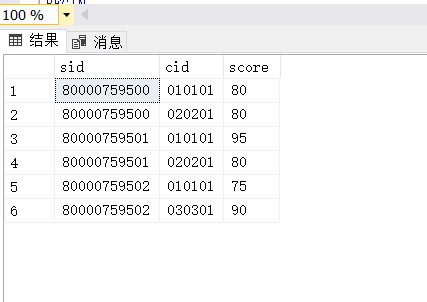
\includegraphics[width=0.9\textwidth]{images/7.png}
  \end{subfigure}
\end{figure}
\inputminted[firstline=118,lastline=174]{sql}{../code/1.sql}

  \item 查询学号为800007595的学生的email转换成大写输出,并查询其选修课程名的前三个字符。提示:使用UPPER()函数和SUBSTRING()函数。
\inputminted[firstline=178,lastline=182]{sql}{../code/1.sql}
\begin{figure}[h]
  \centering
  \caption{运行结果}
  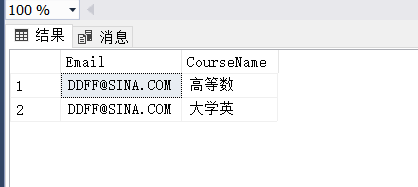
\includegraphics[width=0.4\textwidth]{images/8.png}
\end{figure}
  \item 用户自定义函数分为:标量值函数、内联表值函数、多语句表值函数。实验要求:创建标量值函数,要求根据输入的学生学号参数,返回学生的选课的平均成绩。
\inputminted[firstline=186,lastline=227]{sql}{../code/1.sql}
\begin{figure}[h]
  \centering
  \caption{运行结果}
  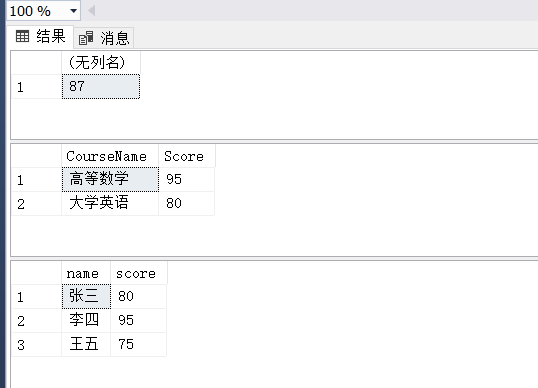
\includegraphics[width=0.4\textwidth]{images/9.png}
\end{figure}

\begin{table}[!ht]
  \centering
  \caption{存储过程和存储函数的异同点和相同点}
  \renewcommand{\arraystretch}{1.5}
  \begin{tabularx}{\linewidth}{@{}|X|X|X|@{}}
    \hline
    类型 & 存储过程 & 存储函数 \\
    \hline
    用途 & 用于执行一系列的T-SQL语句,可以进行数据处理,如插入、删除和更新数据等 &
      用于计算一个单一的数值或结果集并返回该值或结果集 \\\hline
    返回值 & 存储过程可以返回多个结果集 & 存储函数只能返回单一的标量值或结果集 \\\hline
    输入参数 & 存储过程支持默认值,可以使用 `OUTPUT` 修饰符来暴露参数 &
      存储函数必须拥有至少一个输入参数 \\\hline
    输出参数 & 可以定义输出参数,并将它们用作返回值和在存储过程执行结束时传递到调用程序 & 
      不支持输出参数 \\\hline
    异常处理 & 存储过程可以使用 `TRY...CATCH` 结构来处理异常 &
      存储函数不能包含异常处理 \\\hline
    执行计划 & 存储过程在第一次执行时会编译和缓存,可以提高代码的执行性能 &
      存储函数也会编译和缓存,但如果函数中使用了可变数据,该函数不会缓存执行计划 \\\hline
    调用方式 & 存储过程可以通过 `EXEC` 命令或存储过程名称调用 &
      存储函数可以直接在查询中使用,也可以通过函数名称调用 \\\hline
    事务处理 & 存储过程可以在事务中执行,并可以使用事务控制语句 & 存储函数不能用于处理事务 \\\hline
    可重用性 & 存储过程可以设计为可重用的代码模块 & 存储函数也可以设计为可重用的代码模块 \\\hline
    安全性 & 存储过程可以设置安全性,包括权限和角色 & 存储函数也可以设置安全性,包括权限和角色 \\
    \hline
  \end{tabularx}
  \label{tab:storedprocedurefunctioncompare}
\end{table}

  \item 游标不同于查询语句,查询语句只能参整个结果集进行同一种操作,而游标允许定位在结果集的特定行,从结果集的当前位置检索一行或多行,支持对结果集中当前位置的行进行数据修改,为由其他用户对显示在结果集中的数据库数据所做的更改提供不同级别的可见性支持,提供脚本、存储过程和触发器中用于访问结果集中数据的T-SQL语句。
  \begin{quote}
    实验要求:定义一个游标,将学号为800007595的学生的选修课程名和成绩逐行打印出来。
定义一个游标,将学号为800007595的学生的第二门选修课程成绩(成绩降序排列)改为75分。
创建一个没有唯一索引的表,定义一个游标,删除其中一条记录,查看是否允许删除。
  \end{quote}
  \inputminted[firstline=235,lastline=256]{sql}{../code/1.sql}
  \begin{figure}[h]
    \centering
    \caption{运行结果}
    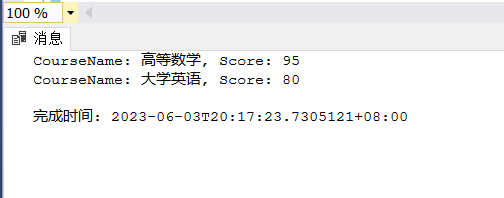
\includegraphics[width=0.4\textwidth]{images/10.png}
  \end{figure}
  \inputminted[firstline=260,lastline=281]{sql}{../code/1.sql}
  \begin{figure}[h]
    \centering
    \caption{运行结果}
    \begin{subfigure}{0.4\textwidth}
      \caption{修改前}
      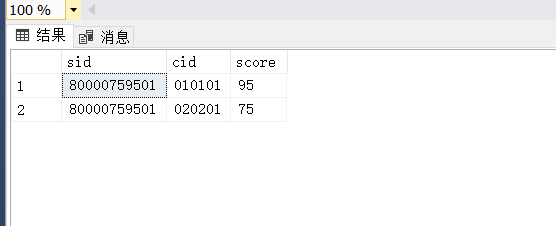
\includegraphics[width=0.9\textwidth]{images/12.png}
    \end{subfigure}
    \begin{subfigure}{0.4\textwidth}
      \caption{修改后}
      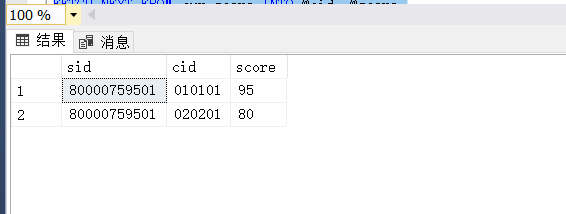
\includegraphics[width=0.9\textwidth]{images/11.png}
    \end{subfigure}
  \end{figure}
  \inputminted[firstline=285,lastline=310]{sql}{../code/1.sql}
  \begin{figure}[h]
    \centering
    \caption{运行结果}
    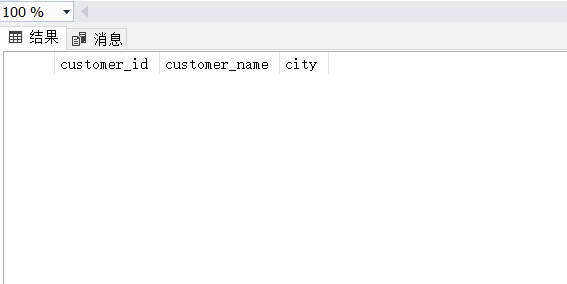
\includegraphics[width=0.4\textwidth]{images/13.png}
  \end{figure}
  可见是可以修改的。
\end{enumerate}

\section{实验总结}

通过本次实验,我学到了数据库管理系统中过程语言的基本概念与语法以及如何使用过程语言进行高效的数据库操作。

在实验过程中,我掌握了变量定义与声明的方法,灵活运用@@ERROR、@@ROWCOUNT、@@IDENTITY等全局变量处理异常。
同时,我还学习了多种流程控制语句的使用方法,例如BEGIN…END、IF…ELSE…、WHILE…CONTINUE…BREAK…、CASE等等,
运用这些语句可以轻松实现复杂的数据处理功能。

此外,我还了解了存储过程的概念,
学习了如何创建存储过程以及如何优化存储过程的性能。
同时,我也学习了如何使用系统函数和用户自定义函数,
这些函数可以极大地简化代码,提高操作效率。

最后,掌握游标的使用也是本次实验的一个重要内容。
我学习了如何在过程语言中使用游标,并灵活应用游标处理数据。

综上所述,此次实验让我对数据库系统的管理和操作有了更深入的了解,
掌握了使用过程语言进行高效的数据库操作的方法和技巧,
也加深了对于数据库系统的学习和理解。

\end{spacing}

\end{document}